\chapter{Sheafification, monodromy}

\section{Sheaf/space adjunction (continued)}
\remyquote{Computers don't have noses.}
\noindent
We still have to prove that the counit of the sheaf/space adjunction is an isomorphism for local homeomorphisms to prove the equivalence $\catSheaf(X)\simeq\catLocalHomeomorphism_{/X}$.

\begin{proof}[of the restricted equivalence in \cref{thm:sheaf-space-adjunction}, continued]
If $f\colon Y\to X$ is a local homeomorphism, we have to show that the counit
\[ \epsilon_{Y/X} \colon \etalespace(h_{Y/X}) \to Y \]
is an isomorphism in $\catLocalHomeomorphism_{/X}$ (or $\catTopologicalSpace_{/X}$).
Concretely, this map is given by
\begin{equation*}
    \begin{tikzcd}[column sep=small]
        \coprod_{U\subseteq X}\cont[X](U,Y)\times U \ar[rr] \ar[rd, epi] & & Y \\
        & \etalespace(h_{Y/X}) \ar[ru, "\epsilon_{Y/X}"']
    \end{tikzcd}
\end{equation*}
where the top map sends $(s,x)_U$ to $s(x)\in Y$.
This map indeed descends to the étalé space $\etalespace(h_{Y/X})$: if $x\in U\subseteq V$ and $s\colon V\to Y$ is a section, then $(s,x)_V\sim(s|_U,x)_U$, and both are sent to $s(x)$.

By \cref{lem:localhomtriangle,lem:etalelocalhomeo}, the map $\etalespace(h_{Y/X})\to Y$ is a local homeomorphism, so in particular an open map, so it suffices to check that it is bijective.

For injectivity, assume $\epsilon_{Y/X}([s,x]_U)=\epsilon_Y([t,y]_V)$.
Then $x=y$ since everything is over $X$, and thus \(s(x)=t(x)\) by assumption.
Let \(S\) be an open neighbourhood of \(s(x)=t(x)\) in \(Y\) such that \(f\) restricts to a homeomorphism \(f|_S\colon S\to f(S)\), and set \(W\coloneq s\inv(S)\cap t\inv(S)\).
Observe that \(W\) contains \(x\).
Then \(s|_W\) and \(t|_W\) are both sections to the injective map \(f|_S\colon S\hookrightarrow X\), so they agree.
Hence \((s,x)_U\approx(s|_W,x)_W=(t|_W,x)_W\approx(t,x)_V\) and we conclude that \(\epsilon_{Y/X}\) is injective.

For surjectivity, let \(y\in V\) and set \(x=f(y)\in X\).
Choose an open neighbourhood \(V\subseteq Y\) of \(y\) such that \(f\) restricts to a homeomorphism \(f|_V\colon V\to f(V) \eqcolon U\) onto an open subset.
Write \(s\colon U\to V\) for its inverse \(f|_V\inv\); then \(s\colon U\to V\subseteq Y\) is a section with \(s(x)=y\), so \(\epsilon_{Y/X}([s,x]_U)=y\), showing that \(\epsilon_{Y/X}\) is surjective.

We conclude that the counit of the sheaf/space adjunction is an isomorphism for local homeomorphisms, finishing the proof of the equivalence of categories \(\catSheaf(X)\simeq\catLocalHomeomorphism_{/X}\) of \cref{thm:sheaf-space-adjunction}.
\end{proof}

\begin{defn}
For a space $X$, the composite functor
\[ (-)^\sharp \coloneq h_{-/X} \circ \etalespace* \colon \catPresheaf(X)\to\catSheaf(X) \]
is called \indexdefnemph{sheafification}.
It comes with a natural map $F\To F^\sharp$ for presheaves $F$ on $X$ given by the unit of the adjunction $\etalespace*\leftadj h_{-/X}$.
\end{defn}

The following result can be seen as the universal property of sheafification\index{sheafification!universal property}.

\begin{cor}\label{cor:sheafification-left-adjoint-to-inclusion}
Sheafification is left adjoint to the inclusion $\catSheaf(X)\hookrightarrow\catPresheaf(X)$.
That is, if $F$ is a presheaf on $X$ and $\mathcal G$ is a sheaf on $X$, then every map $F\To \mathcal G$ of presheaves factors uniquely through the natural map $F\To F^\sharp$.
\end{cor}
\begin{proof}
Compose the adjunction $\etalespace*\leftadj h_{-/X}$ and the equivalence $\catLocalHomeomorphism_{/X}\simeq\catSheaf(X)$.
\end{proof}

The unit of the adjunction is the map $F\To F^\sharp$; it is an isomorphism if and only if $F$ is a sheaf.

\begin{exmp}\label{exmp:sheaf-on-point-set}
For the one-point space $*$, we have $\open(*) = \{\emptyset\hookrightarrow *\}$, so
\[ \catPresheaf(X) = \catFunctor(\mathord{\to},\catSet) \]
is the arrow category of $\catSet$.
As we have seen in the homework, a presheaf $F$ on the one-point space -- that is, a map $F(*)\to F(\emptyset)$ -- is a sheaf if and only if $F(\emptyset)=*$.
Hence we have an equivalence $\catSheaf(X)\simeq\catSet$.
Of course, we also have $\catLocalHomeomorphism_{/*} \simeq\catSet$ since having a local homeomorphism $X\to *$ implies $X$ is discrete.
\end{exmp}

\begin{exmp}
Let $S=\{0,1\}$ be the \indexterm{Sierpiński space} with
\[ \open(S) = \{\emptyset\hookrightarrow\{1\}\hookrightarrow S\}\text{.} \]
Using a similar argument as in the previous example, we see
\[ \catPresheaf(S) \simeq \catFunctor(\mathord{\to}\mathord{\to},\catSet) \]
and
\[ \catSheaf(S) \simeq \catFunctor(\mathord{\to},\catSet)\text{.} \]
\end{exmp}

\begin{exc}
Check that sheafification on $S$ is given by sending a presheaf $F$ -- that is, a pair of maps $F(S)\to F(\{1\})\to F(\emptyset)$ -- to the sheaf given by the map $F(S)\to F(\{1\})$.
\end{exc}

\section{Restriction of sheaves}
\remyquote{You can do this for different values of four, here we do it for five.}

\begin{defn}
Let $U\subseteq X$ be open and let $F$ be a presheaf on $X$.
Then the \emph{restriction}\index{restriction!of sheaves} $F|_U$ of $F$ to $U$ is the restriction of the functor $F$ along the inclusion $\open(U)\hookrightarrow\open(X)$.
\end{defn}

\begin{lem}
If $\mathcal F$ is a sheaf on $X$, then so is its restriction $\mathcal F|_U$ to an open $U\subseteq X$.
Under the equivalence $\catSheaf(X)\simeq\catLocalHomeomorphism_{/X}$, restriction to $U$ corresponds to sending a local homeomorphism $f\colon Y\to X$ to the \indexterm{pullback} $f\inv(U)\to U$.
\end{lem}

In $\catLocalHomeomorphism_{/X}$, we have the subcategory $\catCoveringSpace_{/X}$ of \emph{covering spaces}\index{covering space}: continuous maps $f\colon Y\to X$ such that $X$ has an open cover $X = \bigcup_{i\in I}U_i$ and there are sets $S_i$ such that $f\inv(U_i)\to U_i$ is isomorphic to $U_i\times S_I\to U_i$ (where $S_i$ has the discrete topology) over $U_i$ for all $i\in I$.

\todo{Pancake example}

\begin{rmk}
We will not assume that the space $Y$ in a covering space $Y\to X$ is (path) connected; this condition does appear in the literature with some authors.
\end{rmk}

\begin{defn}
A sheaf $\mathcal F$ on a space $X$ is \emph{locally constant}\index{sheaf!locally constant} if there is an open cover $X = \bigcup_{i\in I}U_i$ such that the restriction $\mathcal F|_{U_i}$ is a constant sheaf $h_{S_i}$ for some set $S_i$ for all $i\in I$.

We write $\catLocallyConstantSheaf(X)$ for the full subcategory of $\catSheaf(X)$ on the locally constant sheaves.
\end{defn}

\begin{lem}
Under the equivalence $\catSheaf(X)\simeq\catLocalHomeomorphism_{/X}$, the locally constant sheaves correspond to covering spaces.
In other words, this equivalence restricts to an equivalence
\[ \catLocallyConstantSheaf(X) \simeq \catCoveringSpace_{/X}\text{.} \]
\end{lem}

The real content is the constant case: we have $\mathcal F\cong h_S = h_{X\times X/X}$ if and only if $\etalespace(\mathcal F)\cong X\times S$ over $X$.
% \begin{proof}
% First, let $\mathcal F$ be a locally constant sheaf on $X$.
% Then there is an open cover $X = \bigcup_{i\in I}U_i$ such that $\mathcal F|_{U_i}\cong h_{S_i}$ for some set $S_i$ for all $i\in I$.
% \end{proof}

\todo{Four-to-one cover of the circle example}

\section{Review of monodromy}
\remyquote{If you've ever been in a parking garage, you know what I mean.}

\begin{figure}[h!]
  \centering
  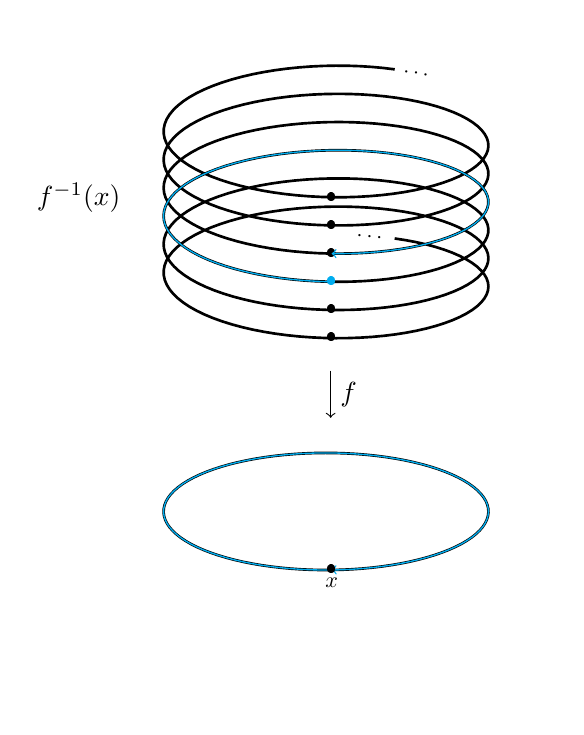
\begin{tikzpicture}[scale=.8]
    \begin{axis}[axis line style={draw=none}, tick style={draw=none}, xticklabel=\empty, yticklabel=\empty, zticklabel=\empty]
      \addplot3+[domain=0:12*pi,samples=500,samples y=0,black,no marks,very thick]
        ({sin(deg(x))}, {cos(deg(x))}, {6*x/(pi)})
        node[pos=0, left, rotate=-5] {\ldots}
        node[pos=1, right, rotate=-10] {\ldots}
        node[pos=0.85/12] {\textbullet}
        node[pos=2.85/12] {\textbullet}
        node[pos=6.85/12] {\textbullet}
        node[pos=8.85/12] {\textbullet}
        node[pos=10.85/12] {\textbullet};
      \addplot3+[domain=4.85*pi:6.85*pi,samples=500,samples y=0,cyan,no marks,semithick,->] ({sin(deg(x))}, {cos(deg(x))}, {6*x/(pi)}) node[pos=0] {\textbullet};
    \end{axis}
    \node at (-0.5,3) {\(f^{-1}(x)\)};
    \draw[->] (3.5,.25) -- (3.5,-0.5) node[right] at (3.5,-0.125) {\(f\)};
    \begin{axis}[axis line style={draw=none}, tick style={draw=none}, xticklabel=\empty, yticklabel=\empty, zticklabel=\empty, at={(0,0,-300)}]
      \addplot3+[domain=0.85*pi:2.85*pi,samples=100,samples y=0,black,no marks,very thick]
        ({sin(deg(x))}, {cos(deg(x))}, {0});
      \addplot3+[domain=0.85*pi:2.85*pi,samples=100,samples y=0,cyan,no marks,semithick,->]
        ({sin(deg(x))}, {cos(deg(x))}, {0})
        node[pos=0,black] {\textbullet}
        node[pos=0,black,below] {\(x\)};
    \end{axis}
  \end{tikzpicture}
  \caption{Unique path lifting in the cover of the circle by the helix}
  \label{fig:unique-path-lifting-circle-helix}
\end{figure}

\begin{defn}
    Let $X$ be a topological space. Then $X$ is 
    \begin{enumerate}
        \item \emph{locally path connected} if every open neighbourhood $x \in U$ of any $x \in X$ contains a path connected open neighbourhood $x \in V \in U$.
        \item \emph{semi-locally path connected} if for every $x \in X$, there exists an open neighbourhood $x\in U$ such that the map $\homotopy[1](U, x) \to \homotopy[1](X,x)$ is trivial. 
    \end{enumerate}
\end{defn}

\begin{defn}
    Let $X$ be a topological space and $x\in X$. The \indexdefnemph{fibre functor} is defined by
    \begin{align*}
        F_x: \catCoveringSpace_{/X} &\to \homotopy[1](X,x)\catSet\\
        (Y \xrightarrow{f} X) &\mapsto f^{-1}(x),
    \end{align*}
    where a loop $\gamma \in \homotopy[1](X,x)$ acts on $f^{-1}(x)$ by unique path lifting. 
\end{defn}

\begin{thm}[name={\indexterm{monodromy} correspondence}]
    Let $X$ be a topological space and $x \in X$. 
    \begin{enumerate}
        \item If $X$ is path connected and locally path connected, then
        \[
            F_x: \catCoveringSpace_{/X} \to \homotopy[1](X,x)\catSet
        \] is fully faithful. 
        \item If $X$ is moreover semi-locally simply connected, then $F_x$ is an equivalence of categories. 
    \end{enumerate}
\end{thm}
\begin{proof}[outline]\todo{Maybe type up the details Marcel}
    \begin{itemize}
        \item Any covering $f: Y \to X$ is locally path connected (easy). It is furthermore a disjoint union $\coprod_{i \in I} Y_i$ of path connected spaces $Y_i$ \cite[Theorem~25.4]{MunkresTopology}.
        \item Any map $Y \xrightarrow{\phi}Y' \in \catCoveringSpace_{/X}$ is itself a covering \cite[Lemma~80.2(a)]{MunkresTopology}.
        \item $F_x$ is faithful: if two maps 
        \[
            \begin{tikzcd}
                Y \arrow[rr, "\phi'"', shift right] \arrow[rr, "\phi", shift left] \arrow[rd, "f"'] &   & Y \arrow[ld, "f'"] \\
                & X & 
            \end{tikzcd}
        \] agree on $f^{-1}(x)$ then they agree: for $y \in Y$ arbitrary, choose a path $\gamma$ starting at $f(y)$ and ending at $x$. By unique path lifting, this gives a path $\overline{\gamma}$ from $y$ to $y'$ for some $y' \in f^{-1}(x)$. Then $\phi(\overline{\gamma})$ and $\phi'(\overline{\gamma})$ are both lifts of $\gamma$ to paths ending at $\phi'(y') = \phi(y')$ so by uniqueness they are the same path and their starting points are the same, i.e. $\phi(y) = \phi'(y)$. 
        \item That $F_x$ is full follows from the lifting lemma \cite[Lemma~79.1]{MunkresTopology}.
        \item $F_x$ is essentially surjective if $X$ is semi-locally simply connected: every $S \in \homotopy[1](X,x)\catSet$ is $S \cong \cup_{i\in I}S_i$ where $\homotopy[1](X,x)$ acts transitively on $S_i$. \todo{explain} Then \[
            S_i \cong \homotopy[1](X,x) / H_i
        \] for $H_i = \text{Stab}(s_i)$ for any $s_i \in S_i$. There exists a covering $Y_i \xrightarrow{f_i} X$ with $\homotopy[1](Y_i, y_i) \xhookrightarrow{} \homotopy[1](X,x)$, one subgroup $H_i$ \cite[Theorem~82.1]{MunkresTopology}, so $S_i \cong F_x(Y_i \xrightarrow{f_i} X)$ and $S = F_x(\coprod_{i \in I} Y_i \to X)$.
        \end{itemize}
\end{proof}
\begin{exmp}
Let $X = S^1$. Let $Y_1$ be the four-to-one covering of $S^1$, and let $Y_2$ be the double covering of $S^1$. Let $Y = Y_1 \coprod Y_2$. Then $Y \to X$ corresponds to the set $\{1,2,3,4,5,6\}$ where the single loop around the circle $1\in \homotopy[1](S^1, x)$ acts by $(12)(3456)$ \todo{Diagram below should have labels etc}.
\begin{figure}
\centering
% https://tex.stackexchange.com/a/495715
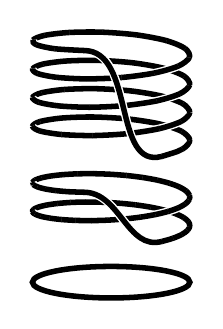
\begin{tikzpicture}[declare function={f(\x)=0.2*sin(\x)+\x/1000;},
 rubout/.style={/utils/exec=\tikzset{rubout/.cd,#1},
 decoration={show path construction,
      curveto code={
       \draw [white,line width=\pgfkeysvalueof{/tikz/rubout/line width}+2*\pgfkeysvalueof{/tikz/rubout/halo}] 
        (\tikzinputsegmentfirst) .. controls
        (\tikzinputsegmentsupporta) and (\tikzinputsegmentsupportb)  ..(\tikzinputsegmentlast); 
       \draw [line width=\pgfkeysvalueof{/tikz/rubout/line width},shorten <=-0.1pt,shorten >=-0.1pt] (\tikzinputsegmentfirst) .. controls
        (\tikzinputsegmentsupporta) and (\tikzinputsegmentsupportb) ..(\tikzinputsegmentlast);  
      }}},rubout/.cd,line width/.initial=2pt,halo/.initial=0.5pt]
 \draw[rubout={line width=2pt,halo=0.5pt},decorate] 
   plot[variable=\x,domain=-50:1330,samples=55,smooth] ({cos(\x)},{f(\x)}) to[out=0,in=195] cycle;
 \draw[rubout={line width=2pt,halo=0.5pt},decorate] 
   plot[variable=\x,domain=-1130:-470,samples=55,smooth] ({cos(\x)},{f(\x)}) to[out=0,in=195] cycle;

 \draw[line width=2pt] (0,-2) arc(-90:270:1cm and 0.2cm);
 % \draw[thick,-stealth]  (0,-0.4) -- (0,-1.4) node[midway,right]{$p$};
\end{tikzpicture}
\caption{Covering of the circle by a disjoint union of the four-to-one cover and the two-to-one cover.}
\label{fig:circle-cover-quadruple-double}
\end{figure}
\end{exmp}

The following diagram summarises the situation if $X$ is a `nice' space:
\begin{equation*}
    \begin{tikzcd}
        \catSheaf(X) \ar[r, "\simeq"] & \catLocalHomeomorphism_{/X} \\
        \catLocallyConstantSheaf(X) \ar[u, inclusion] \ar[r, "\simeq"'] & \catCoveringSpace_{/X} \ar[u, inclusion] \ar[r, "\simeq"'] & \homotopy[1](X,x)\catSet
    \end{tikzcd}
\end{equation*}
This diagram raises the question: what should there be in the top right spot?
Towards the end of the course, we will give a partial answer which goes by the name of \emph{exodromy}.